\begin{tips}
    直线只研究方向向量，平面只研究法向量。
\end{tips}

\begin{theorem}[叉乘法求法向量]
    设 $\overrightarrow{A B}, \overrightarrow{A C}$ 是平面 $A B C$ 的两个不共线的向量，则平面 $A B C$ 的法向量可以用叉乘法。

    具体的操作是：求谁盖谁，Y 加负号。
\end{theorem}

\section{异面直线所成的角}

\subsection{通过平移与余弦定理构造}



\subsection{通过建系求解}



\begin{theorem}

\end{theorem}

\section{空间中的动点和距离问题}

\begin{problem}
如图，在三棱锥 $A-B C D$ 中，$\triangle A B C$ 是正三角形，平面 $A B C \perp$ 平面 $B C D, ~ B D \perp C D$ ，点 $E, ~ F$ 分别是 $B C, ~ D C$ 的中点．
\begin{enumerate}
    \item[(1)] 证明：平面 $A C D \perp$ 平面 $A E F$ ；
    \item[(2)] 若 $\angle B C D=60^{\circ}$ ，点 $G$ 是线段 $B D$ 上的动点，问：点 $G$ 运动到何处时，平面 $A E G$ 与平面 $A C D$ 所成的锐二面角最小．
\end{enumerate}

\begin{figure} [H]
    \centering
    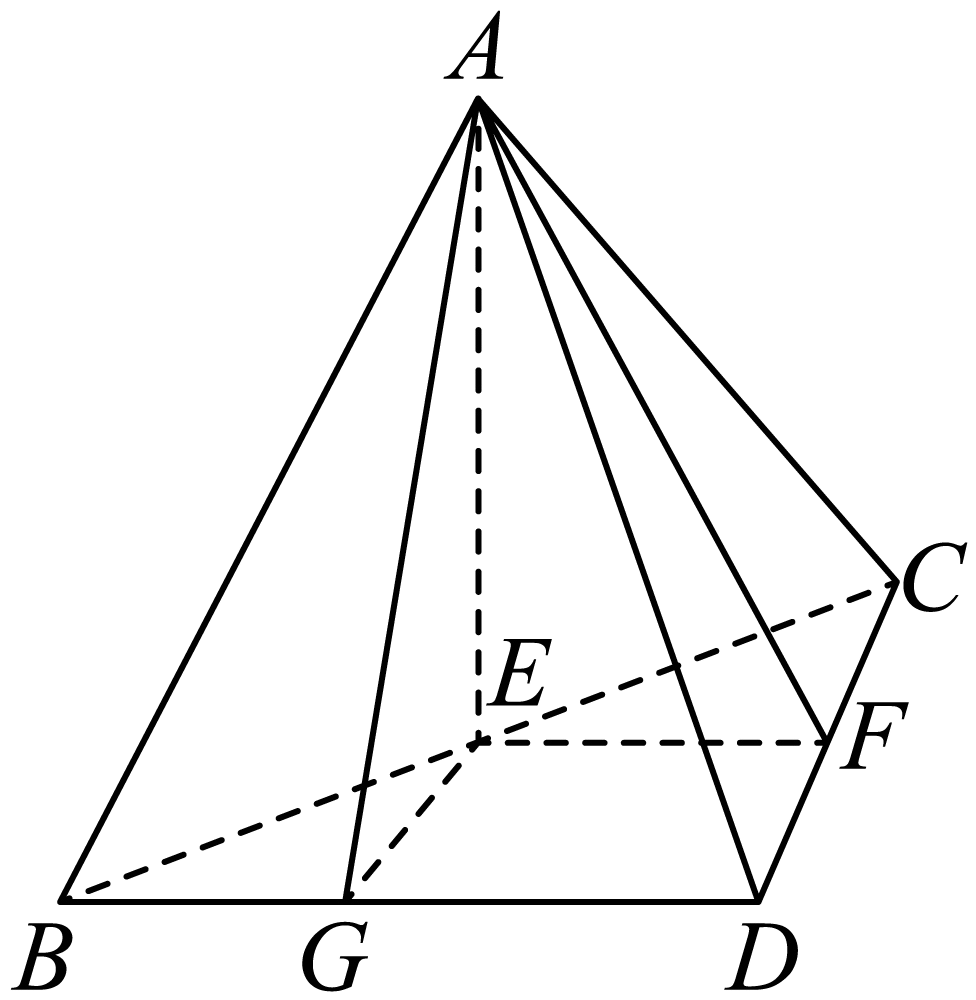
\includegraphics[width=0.2\textwidth]{chapters/solid-geometry/images/建系法求角/img-20250704221209.png}
\end{figure}

\end{problem}

\subsection{线面角与点面距的计算}

\begin{problem}
如图，在四棱柱 $A B C D-A_1 B_1 C_1 D_1$ 中，$A A_1 \perp$ 平面 $A B C D$ ，底面 $A B C D$ 是平行四边形，$A B=A D=B D=A A_1=2$ 。
\begin{enumerate}
    \item[(1)] 求直线 $B D_1$ 与平面 $A C D_1$ 所成角的正弦值；
    \item[(2)] 求点 $B_1$ 到平面 $A C D_1$ 的距离．
\end{enumerate}

\begin{figure} [H]
    \centering
    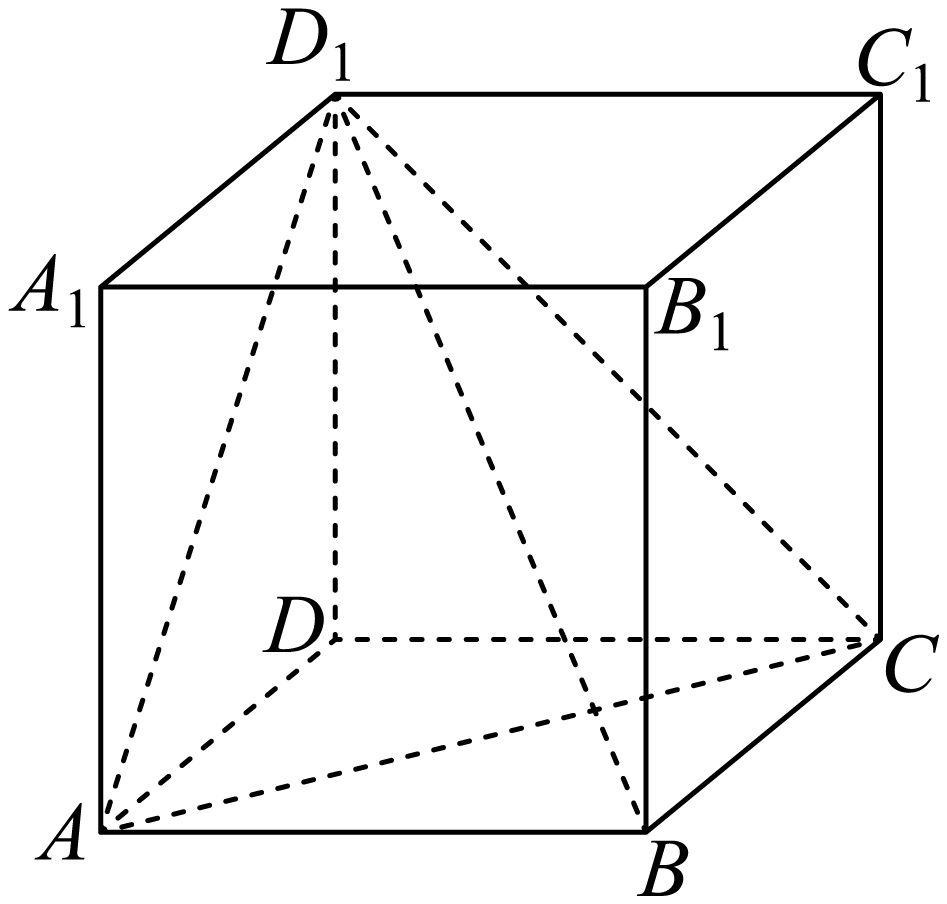
\includegraphics[width=0.2\textwidth]{chapters/solid-geometry/images/建系法求角/img-20250704221316.png}
\end{figure}

\end{problem}

\subsection{平面法向量与存在性问题}

\begin{problem}
如图，在四棱雉 $P-A B C D$ 中，$B D \perp P C, ~ \angle B A D=120^{\circ}$ ，四边形 $A B C D$ 是菱形，$P B=\sqrt{2} A B=\sqrt{2} P A, ~ E$ 是棱 $P D$ 上的动点，且 $\overrightarrow{P E}=\lambda \overrightarrow{P D}$.
\begin{enumerate}
    \item[(1)] 证明：$P A \perp$ 平面 $A B C D$ ；
    \item[(2)] 建立适当的空间直角坐标系，求面 $P A B$ 法向量和平面 $A C E$ 的法向量；
    \item[(3)] 是否存在实数 $\lambda$ ，使得平面 $P A B$ 与平面 $A C E$ 的夹角的余弦值是 $\frac{\sqrt{7}}{7}$ ？若存在，求出 $\lambda$ 的值；若不存在，请说明理由．
\end{enumerate}

\begin{figure} [H]
    \centering
    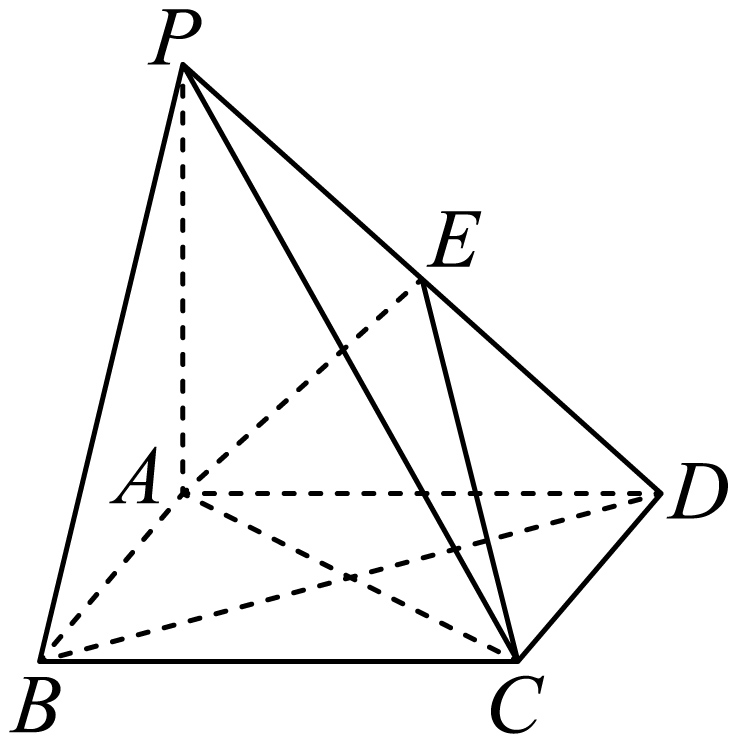
\includegraphics[width=0.2\textwidth]{chapters/solid-geometry/images/建系法求角/img-20250704221453.png}
\end{figure}
\end{problem}